\documentclass{article}
\usepackage[margin=1in]{geometry}
\usepackage{graphicx}
\title{Boids!}
\author{Homework \#1, CSCI 322, Winter 2016}
\date{}
\begin{document}
\maketitle
\centerline{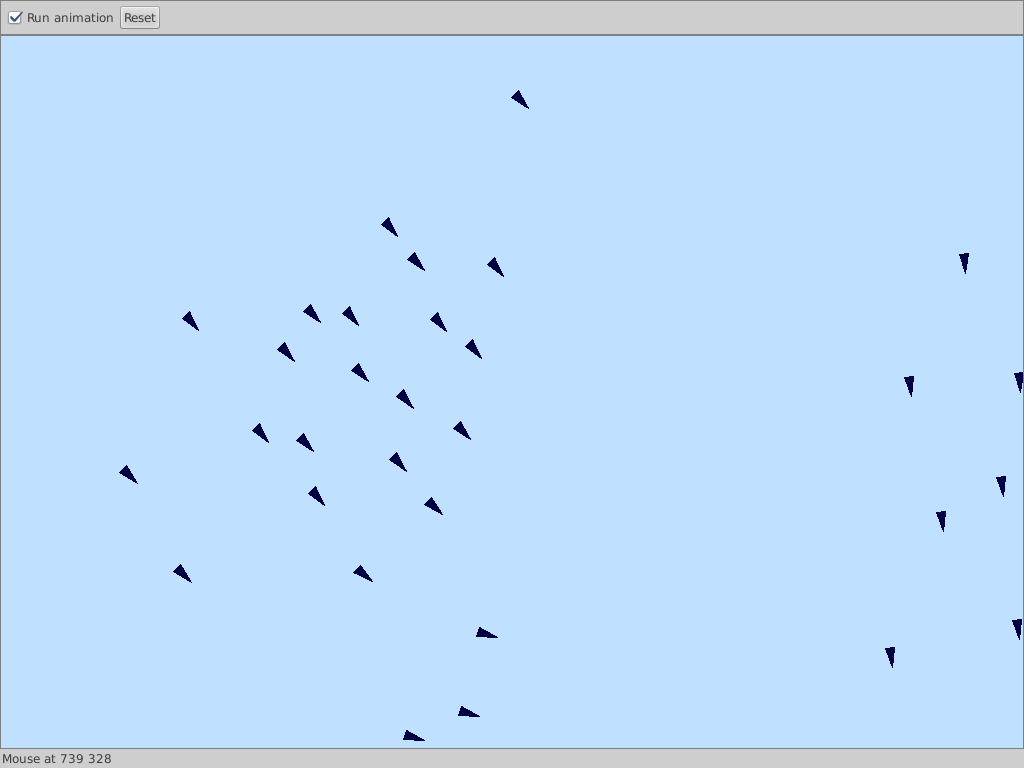
\includegraphics[width=0.5\textwidth]{boids.png}}
\begin{description}
\item[Demo boids:]  I have placed an animated boids demo in the class
  repo called {\tt boids00.rkt}.  Currently it uses no explicit
  threading, tha animation loop uses busy waiting when there is no
  animation, and it uses {\tt sleep/yield} in order to collaborate
  with the GUI.
\item[Project:]
  Create two new versions of this program:
  \begin{enumerate}
\item A program called {\tt boids01.rkt} that uses a single thread
  for the animation loop:  calculate forces, move the boids, refresh
  the view, sleep, repeat.
  \begin{itemize}
    \item Clicking the checkbox should suspend and
  resume this thread. \item There should be no busy waiting when the
  animation is suspended.  \item Use {\tt sleep } instead of {\tt
    sleep/yield}.
\item
  Also, kill (not suspend) the animation thread when the window is
  closed.  You do this by augmenting the {\tt on-close} method of the
  top level {\tt frame\%}.  See my {\tt onclose.rkt} example in the
  repo.  (You may notice that my version does not quit properly.)
\end{itemize}
\item A program called {\tt boids02.rkt} that uses a new thread for
  each new boid.
  \begin{itemize}
  \item Each thread will take care of calculating the
  forces and updating the position of its own boid.
\item
  Every time the mouse is clicked, a new boid and a new thread are
  created. The new threads should be contained in the boid objects
  themselves (a new field in the object).
\item
  There should be one more thread that takes care of refreshing the
  view (there’s no point in each boid refreshing the view). Note that
  the view refreshing does not have to happen at the same frequency as
  the boid updating. For example, given enough cycles, we can update
  the boid positions more frequently than we refresh the view, to get
  a more accurate simulation.
\item
  Clicking the checkbox suspends and resumes all of these
  threads.
  \item Again, no busy waiting and no sleep/yield.
\item
  Also, kill all
  threads when the window is closed.
  \end{itemize}
  \end{enumerate}


\item[Due date:] Monday, January 25, at
  midnight. Remember to upload both programs. Each should be stand-
  alone and run without the other. 50\% of this assignment's grade
  points for each stage.
  

\end{description}

\end{document}
